\chapter{Introduction}
\label{sec:intro}

\acp{MAV} are an emerging technology that support society in a wide range of consumer, industrial and safety applications. For example \acp{MAV} are used to deliver medicine\cite{Shankland2018}, fight fires \cite{KateBaggaley2017} or even find survivors in disaster situations \cite{JoshuaBateman2017}.

\begin{figure}[b]
	\centering
	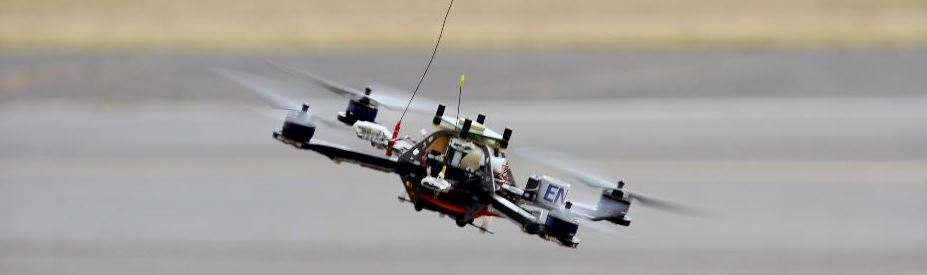
\includegraphics[width=\textwidth]{fig/mav}
	\caption{A Quadrotor-\ac{MAV}}
	\label{fig:mav}
\end{figure}


Especially in emergency scenarios the fast and safe flight of \acp{MAV} is crucial to deliver help quickly and save human lives. However, due to the complexity of such missions as well as the difficulty to control an \ac{MAV} in these kind of scenarios, often multiple human operators are required in order to ensure safe operation \cite{Murphy2016}. With humans in the loop a constant connection between the \ac{MAV} and the operators is required which not only uses energy and requires infrastructure but also significantly reduces the reaction time. Enabling \acp{MAV} to fly more autonomously could allow less human operators to control more \acp{MAV} and thus to improve the support in emergency missions.

A major challenge on the way to the full autonomous flight of \acp{MAV} is the accurate estimation of the \ac{MAV}'s state within its environment. The system is highly dynamic so position and orientation can change rapidly. At the same time noise introduced by motor vibrations makes the position estimation with on-board \acp{IMU} alone too inaccurate \cite{Mohamed2014}. \ac{LIDAR}-sensors can capture long and wide range 3D information but the sensors are typically heavy and require energy. \ac{IR} sensors can cover distance information but are often limited in their \ac{FoV} as well as their range. External infrastructure like \ac{GPS} and optical tracking systems can provide accurate measurements but there is no guarantee that such systems are present in real world applications. Cameras on the other hand are cheap, lightweight and can measure long range distance information. This makes them a suitable choice as a sensor for on-board state estimation on light \acp{MAV}\cite{Elbanhawi2017}.

However, the signal delivered by the camera is high dimensional data that can not directly be interpreted as position or orientation measurement. Further processing by computer vision algorithms is required to interpret the image and extract relevant information. Thereby machine learning based methods are a popular choice to process the signal. Instead of designing an algorithm manually, the image processing is learned by using annotated examples. In particular deep learning based methods aim to combine whole computer vision pipelines into one mapping that transforms the raw input image into task dependent output. Experiments have shown how deep learning based methods outperform traditional machine learning approaches and manually crafted algorithms in a lot of examples \cite{Razavian}. This made them predominant choice for almost any vision task.

\begin{figure}[hbtp]
	\centering
	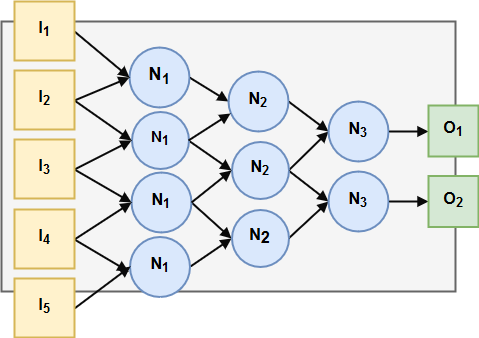
\includegraphics[width=0.6\textwidth]{fig/cnn_example}
	\caption{Simple Example Architecture of a \ac{CNN} with three layers. The input image $I$ is transformed by the nodes $N$ to the desired output $O$. Thereby the parameters of $N$ are learned from annotated examples.}
	\label{fig:cnn_example}
\end{figure}

The hereby used \acp{CNN} are designed in a hierarchical way, using multiple layers that are evaluated sequentially. An example architecture is displayed in \autoref{fig:cnn_example} By stacking more layers on top of each other (deepening) and increasing the number of nodes per layer (widening), highly non-linear functions can be modelled. Various experiments have shown the superior performance of particularly deep/wide models  \cite{He, He2015, Szegedy2014, Zagoruyko2016}. However, this model flexibility assumed to be the reason for their superior performance also leads to immense requirements in computational resources. For example a state-of-the-art image classification system contains TODO multiplications and additions. 

On robotic platforms like \acp{MAV} that have limited resources in terms of processing power and battery life but need to follow real-time constraints the deployment of such methods is still an open challenge. Despite a lot of research that addresses to reduce the number of computations in deep learning models \cite{YoungwanLee, Zagoruyko2016, Howard2017, Ghosh2017, Sandler2018, Zhang2017a} the investigation of relatively shallow models with less than ten layers received only little attention by the research community.

This work investigates the deployment of a deep learning based computer vision pipeline on a \ac{MAV}. The method is applied in the challenging scenario of Autonomous Drone Racing at the \ac{IROS} 2018. Within the race court several metal gates are placed and need to be passed one after another. Detecting the gates, allows to estimate the \ac{MAV}'s relative position and to calculate the flying trajectory. An overview of the race court and the racing gates at the \ac{IROS} 2016 Autonomous Drone Race can be seen in \autoref{fig:race_court}.

\begin{figure}[bhtp]
	\centering
	\begin{minipage}{0.45\linewidth}
	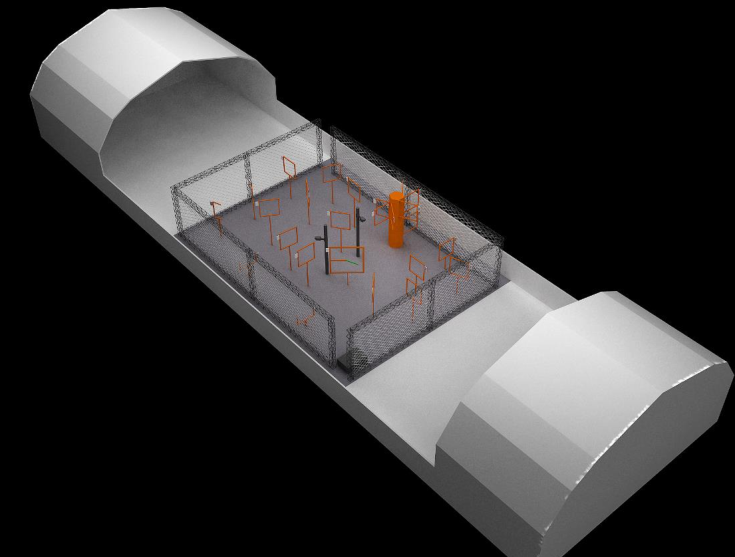
\includegraphics[width=\textwidth]{fig/race_court}
	\end{minipage}\hfill
\begin{minipage}{0.45\linewidth}
	\includegraphics[width=\textwidth]{fig/race_court_side}
\end{minipage}
\caption{Example Images of the \ac{IROS} 2016 Autonomous Drone Race}
\label{fig:race_court}
\end{figure}

In contrast to a lot of objects in the real world that consist of distinct and complex shapes like a pedestrian that consists of body parts and a face, the racing gates consist only of thin edges and corners that are spread over large distances in the image. Additionally a majority of the area covered by the object is transparent and can therefore contain all kind of contents including other objects. This introduces a vision task that even humans have a hard time at solving. The unconvinced reader can try to count the number of gates visible in \autoref{fig:race_court} in the right image.

AsDetecting these kind of objects is particularly challenging for a vision system as distinctive properties can not be easily identified and the gap between the corners can undergo large variations. 

Therefore it is crucial that the annotated examples

 the object shape poses a particular challenge for a vision system. The object class is referred to as empty, wire frame objects and the particular modelling of the detection task is addressed in \autoref{sec:object_detection}. 

Without an accurate detection of the racing gate, the \ac{MAV} is not able to determine its current position and thus to calculate its flying trajectory. On the other hand, with a algorithm that requires less computational resources a lighter \ac{MAV} can be built. This allows faster and more aggressive trajectories as well as longer battery live. Hence, the trade-off between accuracy and inference speed is of particular interest for this application and is addressed in \autoref{sec:tradeoff}.

Another drawback of deep-learning based methods is the requirement of a vast amount of annotated examples which are in this application similar to many others not available. Alternatively, data can be synthesized using graphic engines which allows the generation of theoretically infinite data. The generation of artifical data to train a object detection model is studied in \autoref{sec:training}.

\subsection*{Research Question}

The research question of this work is formulated as follows:
\begin{center}
	\textbf{How can a model for object detection of wire frame objects on \acp{MAV} be learned from synthetic data?}
\end{center}


This question is split into multiple questions that address individual parts of the topic:

\begin{itemize}
	\item How can data be generated to train a detection model for wire frame object detection on \acp{MAV}?
	\item How can a detection model represent wire frame objects?
	\item How can the inference time of a object detector be optimized for the application on a micro-air vehicle?
	\item Can the gained insights be used to build a lightweight and robust detection model for wire frame objects to be applied in autonomous drone racing?
\end{itemize}

Assumptions:
- There is a concept within the images of the race court that is consistent across all images and that can be generalized
- This concept can be extracted from annotated examples

The remaining parts of this thesis are structures as follows: \autoref{sec:evaluation} describes the metrics and systems used for evaluation.\\
 \autoref{sec:training}, \autoref{sec:object_detection} and \autoref{sec:tradeoff} address the individual research questions. Each chapter contains an introduction to the topic and experiments that have been carried out. \autoref{sec:training} describes methods to learn with limited availability of training data. It concludes with the datasets used for the remaining parts of this thesis.  \autoref{sec:object_detection} describes object detection and evaluates current methods in the application for wire frame objects.
\autoref{sec:tradeoff} illustrates and evaluates measures to reduce computations.
\autoref{sec:method} describes the method proposed in this work.\\
\autoref{sec:disc} discusses the overall results and formulates a conclusion.
